\chapter{Overenie riešenia}

Keďže sme natrénovali viacero modelov, ako prvé sme ich porovnali na našej implementácii metódy RISE pre 3D snímky.
Následne sme vybrali z nich najlepší model, na ktorom sme vyskúšali rôzne nastavenia metódy RISEI, pretože skúšanie rôznych parametrov metódy RISEI je časovo náročné.

\section{Experimenty}

\subsection{Porovnanie metódy RISE na natrénovaných modeloch \label{sec:experiment_rise_various_architectures}}

V tomto experiemnte sme porovnali metódu RISE na nami natrénovaných modeloch. Použili sme nami implementovaný metódu RISEI pričom sme nastavili jej parametre tak, aby fungovala ako metóda RISE.
Parametre sme nastavili nasledovne: $s = 8$, $p = 1/3$, $b1 = 0$, $b2 = 1$ (opis parametrov sa nachádza v tabuľke \ref{tab:risei_params}). Pri vyhodnocovaní metrík insertion a deletion sme nastavili veľkosť kroku na 2500 voxelov (takto trvalo vyhodnotenie tepelnej mapy ~3 minúty). Ku 25 snímkom vygenerovalo a vyhodnotilo tepelné mapy za ~1 hodinu. Najlepšie výsledky sme dosiahli na architektúre 3D CNN (Tabuĺka \ref{tab:experiment_rise_various_architectures}).

\begin{table}[]
    \centering
    \begin{tabular}{cl|r|r|r|}
        \cline{3-5}
        \multicolumn{1}{l}{} &  & \multicolumn{1}{c|}{3D CNN} & \multicolumn{1}{c|}{3D ResNET} & \multicolumn{1}{c|}{2D ResNET} \\ \hline
        \multicolumn{1}{|c|}{\multirow{2}{*}{Insertion (AUC)}} & priemer & \textbf{0.50} & 0.46 & 0.38 \\ \cline{2-2}
        \multicolumn{1}{|c|}{}                                 & medián  & \textbf{0.53} & 0.13 & 0.30 \\ \cline{1-2}
        \multicolumn{1}{|c|}{\multirow{2}{*}{Deletion (AUC)}}  & priemer & \textbf{0.53} & 0.81 & 0.62 \\ \cline{2-2}
        \multicolumn{1}{|c|}{}                                 & medián  & 0.60 & 0.83 & \textbf{0.43} \\ \hline
    \end{tabular}
    \caption{\textbf{Porovnanie metódy RISE na rôznych architektúrach.} Pre insertion sú lepšie vyššie hodnoty (očakávame, že keď vložíme najpodstatnejšie voxely aktivácia bude stúpať), pre deletion sú lepšie nižšie hodnoty (očakávame, že keď ostránime najdôležitejšie voxely, aktivácia bude klesať).}
    \label{tab:experiment_rise_various_architectures}
\end{table}

\subsection{RISE vs RISEI}

V tomto experimente sme porovnali RIZE a rôzne nastavenia metódy RISEI. Použili sme 3D CNN model s úspešnosťou 72\%, senzitivitou 73\% a špecificitou 71\%, toto nie je rovnaký model ako ten, ktorý sme použili v predchádzajúcom experimente, ale jeden z prvých modelov, ktorý sme natrénovali. Keďže sme postupovali iteratívne a inkrementálne, snažili sme sa overiť metódu RISEI čo najskôr. Najnovší 3D CNN model sme nestihli použiť v tomto experimente. 

Použili sme rovnaké nastavenie parametrov ako v predchádzajúcom experimente (Sekcia \ref{sec:experiment_rise_various_architectures}) a menili sme len parametre \textit{b1}, \textit{b2} a \textit{b2\_value}. Parametre \textit{in\_paint\_radius} sme nastavili na hodnotu $5$. Vyhodnocovali sme zatiaľ len metriku \textit{insertion}, najlepšie výsledky sme dosiahlli bez použitia dokreslenia ale s prekrytím hodnotou jedna. Obrázok \ref{fig:heatmap_and_auc_example} zobrazuje príklad vygenerovanej tepelnej mapy pre MRI snímok a výsledný graf zmeny aktivácie pre metriky \textit{insertion}.

\begin{table}[]
    \centering
    \begin{tabular}{l|l|l|}
        \cline{2-3}
                                                                    & \multicolumn{2}{c|}{Insertion} \\ \cline{2-3} 
                                                                    & Priemer        & Medián        \\ \hline
        \multicolumn{1}{|l|}{b1 =  0, b2 = 1, b2\_value = min (RISE)} & 0.43           & 0.37          \\ \hline
        \multicolumn{1}{|l|}{b1 =  0, b2 = 1, b2\_value = max}        & \textbf{0.65}  & \textbf{0.67} \\ \hline
        \multicolumn{1}{|l|}{b1 =  0, b2 = 1, b2\_value = median}     & 0.52           & 0.48          \\ \hline
        \multicolumn{1}{|l|}{b1 =  1, b2 = 0}                        & 0.53           & 0.47          \\ \hline
        \multicolumn{1}{|l|}{b1 =  1, b2 = 0.25, b2\_value = min}     & 0.49           & 0.42          \\ \hline
        \multicolumn{1}{|l|}{b1 =  1, b2 = 0.5, b2\_value = min}      & 0.44           & 0.37          \\ \hline
        \multicolumn{1}{|l|}{b1 =  1, b2 = 0.75, b2\_value = min}     & 0.39           & 0.30          \\ \hline
    \end{tabular}
    \caption{\textbf{Porovnanie rôznych nastavení metódy RISEI.} Najlepšie výsledky dosiahla metóda bez použitia dokreslenia ale s prekrytím hodnotou jedna.}
    \label{tab:experiment_risei_various_configuration}
\end{table}

\begin{figure}[h!]
    \centering
    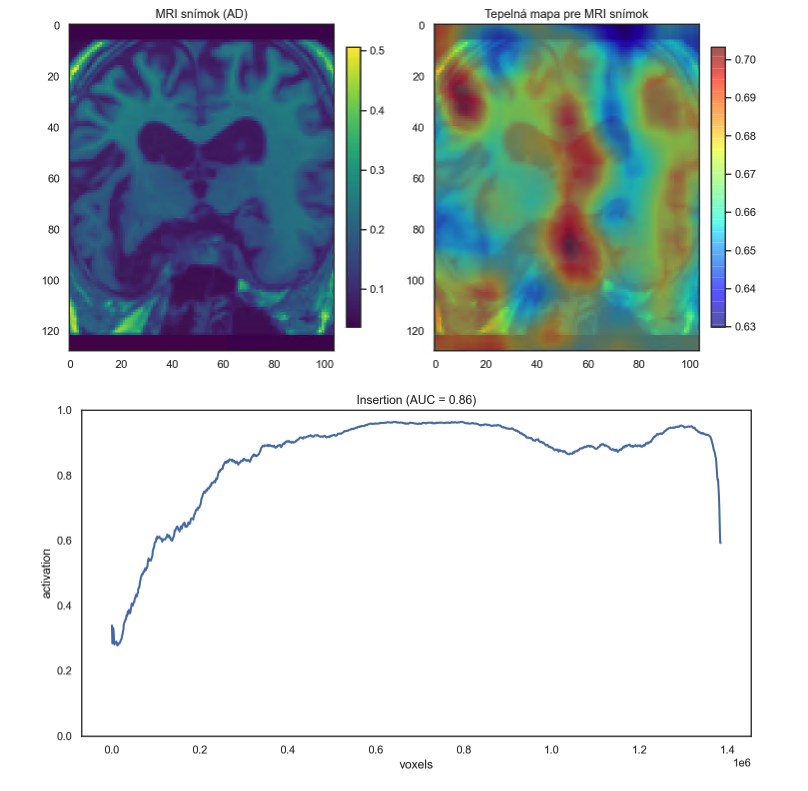
\includegraphics[width=14cm]{assets/images/heatmap_and_auc_example.png}
    \caption{Vygenerovaná tepelná mapa a graf zmeny aktivácie po pridávaní voxelov pre vybraný MRI snímok. Metrika AUC je pomerne vysoká, avšak je potrebné tepelnú mapu ešte vyhodnotiť z pohľadu segmentačných masiek. Tepelná mapa bola vygenerovaná s parametrami \textit{b1 = 1, b2 = 0}.}
    \label{fig:heatmap_and_auc_example}
\end{figure}

Ako možná zmena do ďaľších experimentov je používať hodnotu \textit{max} ako hodnotu pre parameter \textit{b2\_value} v kombinácii s \textit{b1 = 1} a \textit{b2 < 1}, keďže dosiahla zatiaľ najlepšie výsledky.

\section{Záver}

Zistili sme, že metóda RISE s dokresľovaním dosahuje lepšie výsledky ako pôvodná metóda ktorá zakrývala minimálnou hodnotou. Pokial ale minimálnu hodnotu nahradíme maximálnou, dosiahneme lepšie výsledky ako s dokreslovaním, ktoré dosahuje podobné vśyeldky ako zakrývaním mediánom. Avšak, vyhodnocovali sme zatiaľ len pomerne malej vzorke a nebrali sme do úvahy početnosť tried (AD a CN) v tejto vzorke čo je nedostatkom našich experimentov (v ďaľších experimentoch by mali byť tieto triedy vyvážené). Zároveň na dátach z tejto vzorky nemali testované modely 100\%-nú úspešnosť.

Na generovanie tepelných máp sme použili 1000 masiek (keďže autori metódy RISE v experimentoch použili podobný počet), avšak my máme iný typ dát (3D volumetrické dáta), preto je vhodné vyskúšať rôzne počty a nájsť vhodný počet pre náš problém.

Keďže sú masky pri generovaní tepelných máp náhodné, je možné, že pre jeden MRI snímok metóda vygeneruje rôzne tepelné masky. V ďaľších experimentoch by sme mali vyhodnocovať aj konzistenciu tepelných máp - tj. ako veľmi sa líšia medzi rôznymi použitiami metódy na tom istom snímku. Predpokladáme, že väčší počet použitých másk bude viesť ku konzistentnejším tepelným mapám. Takýmto meraním môžeme dospieť k optimálnemu počtu masiek, ktorý je potrebný na generovanie tepelnej mapy.

Taktiež je potrebné vyhodnotiť správnosť tepelných máp vzhľadom na segmentačné masky, tak ako sme uviedli v návrhu riešenia (Sekcia \ref{sec:heat_maps_and_model_segmentation_masks}). Ďalej je potrebné porovnať navrhovanú metódy s inými existujúcimi metódami, napr. LRP alebo analýza senzitivity.


% TODO: we need to compare our method with other methods like LRP or other oclussion methods
% TODO: evaluate the consistency of heatmaps, the method several times for the same image and find out if heatmaps are consistent - this way we can find also optimal number of masks
% TODO: compare with segmentation masks, if more heat is in important areas
